\documentclass[11pt,a4paper,titlepage]{article}

\usepackage{pdflscape}
\usepackage[margin=1in]{geometry}
\usepackage{titling}
\usepackage{graphicx}
\usepackage{titlesec}
\PassOptionsToPackage{hyphens}{url}\usepackage[hidelinks]{hyperref}
\usepackage{datetime}

\graphicspath{ {./Images/} }

\setcounter{secnumdepth}{4}

\titleformat{\paragraph}
{\normalfont\normalsize\bfseries}{\theparagraph}{1em}{}
\titlespacing*{\paragraph}
{0pt}{3.25ex plus 1ex minus .2ex}{1.5ex plus .2ex}

\newdateformat{monthyeardate}{%
  \monthname[\THEMONTH], \THEYEAR}


\begin{document}
%\title{ \huge Functional Requirements for the SAMBUG}

\begin{titlepage}
	
	
	\begin{center}
		\vspace*{-3cm}
  		\makebox[\textwidth]{\includegraphics[width=\paperwidth]{sambug}}
	\end{center}
	
	%\includegraphics[width=\paperwidth]{sambug}
	
    \vspace*{2cm}
      \Huge \textbf {SAMBUG}\\
      
    \vspace*{-0.5cm}
	  \huge \textbf {Architectural Requirements}\\
	  \hfill\\
	\vspace*{-0.5cm}  
      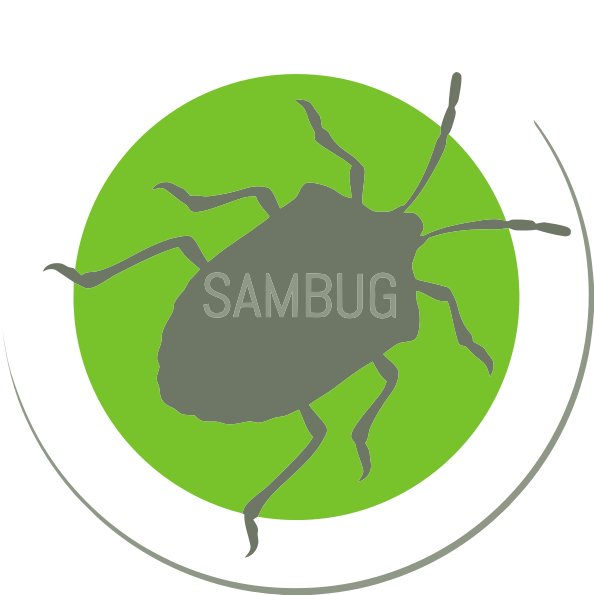
\includegraphics[scale=0.2]{logo}\hfill
	\includegraphics[scale=0.2]{sambug_logo}
         
    \vskip2cm
          
    \large \textbf{\monthyeardate\today}
  
    \vfill
\begin{tabular}{lr}
        	Abrie van Aardt&13178840\\
		Werner Mostert&13019695\\
		Kale-ab Tessera&13048423\\
		Keagan Thompson&13023782\\
		Michelle Swanepoel&13066294\\
	\end{tabular}
\end{titlepage}

	
%\author
%{     
%	Abrie van Aardt 13178840\\
%	Werner Mostert 13019695\\
%	Kele-ab Tessera 13048423\\
%	Keagan Thompson 13023782\\
%	Michelle Swanepoel 13066294\\
%}
    
%\date{\textbf{May 2015}}

%\maketitle

\tableofcontents

\pagebreak


% Put all images in images folder - Please use PNG's not Jpegs
% Preferably create separate file for your domain - just like with the use cases
\pagebreak


		
		
\section{Architectural Requirements}
	\subsection{Quality Requirements}
		\subsubsection{Maintainability}
			As a standard requirement for all projects, SAMBUG needs to be maintainable. This is especially important due to the fact that the project has a very high expansion potential. SUBTROP has shown interest in further maintaining the project after completion.
			Since development on the project is split among 5 members, we have to ensure that the code is as readable as possible and this includes using good documentation of code in the form of comments and inline comment descriptions.
		\subsubsection{Scalability}
			Since the user base for the system will be comparatively small, scalability is not a great issue at this moment in time. The load on the system will not under any foreseeable circumstances be extremely high in the near future. However, it is good practice to cater for the fact that any project, no matter how small, has the potential to grow. Due to this fact, scalable solutions are of high importance. 
		\subsubsection{Performance Requirements}
			Performance is a very important requirement for the system. The goal of the system is to provide an efficiently rendered service. Users of the system will be subject to high pressure environments where time is a limiting factor. Using phone memory effectively is also a must as the phones used by the users might not be latest models, and therefore may struggle with some of the more computationally expensive sub sections of the application.
		\subsubsection{Reliability and Availability}
			Since users will be relying heavily on this system to make important business decisions the system must be available to be used at all times. As such, a reliable system is of paramount importance. The storing of data and persistence of said data to the server must be completely reliable since this is the essential part of the project objectives. 
		\subsubsection{Security}
			As specified by the client, for the sake of reducing usage complexity of the system, the security may be relaxed in this case due to the fact that the users are generally not comfortable with using technological products. However, security measures should be put in place  to provide for a fundamental level of data protection.
		\subsubsection{Auditability}
			Since there is business value in tracking user activity in the form of checking that scouters actually covered a specific area of a farm, auditability is therefore paramount. Auditibility in this case is implicitly obtained by finding the user's coordinates which relates to the specific user who is logged in at the time. 
		\subsubsection{Testability}
			Every service offered by the system should be testable via:\\
			1. Unit tests\\
			2. Integration tests
		\subsubsection{Usability}
			Usability is the main quality requirement for the system. In order for the system to have any actual business value it should be easy to use and effective. As far as possible, the user should be able to use the Application without needing textual instructions. Symbolic icons for action controls are used and to cater for the modernised user, a very well-known interaction flow is used as is common with applications from Google.
		\subsubsection{Deployability}
			The system must be deployable to any cloud hosted, Windows based, virtual machine or locally hosted server.
	\subsection{Architecture responsibilities}
	The architectural responsibilities of the system include providing infrastructure for the following:
		\begin{itemize}
			\item A web access channel
			\item A mobile access channel
			\item Hosting for business logic and services offered by the system
			\item Relational database persistence
			\item Sending emails for recovering of accounts
		\end{itemize}
\section{Architectural Design}
	\subsection{Overview}
		A layered architecture will be used to provide for better decoupling of the various		access channels and architectural responsibilities. Within these layers the Model-View-Controller pattern will be applied to further separate concerns among what can be viewed as three distinct parts of a Web application. The following provides an overview of the architecture:
			\begin{itemize}
				\item Access Layer
					\begin{itemize}
						\item View\\
						In many ways the Android application serves as an access channel to the Web server. However, it is not categorised as a "View" in the MVC sense. Our MVC pattern is only used across the Access and Services layers. Therefore, this only encompasses HTML views that are rendered using the Razor rendering engine.
						\item View Model\\
						Model definitions are used both in the View and in the Controller, since these define the primary format of data transfer between those two components. It is important to remember that since MVC is used solely for the frontend, these models are only view models, and not data or domain models.
					\end{itemize}
				\item Services Layer
				    \begin{itemize}
						\item View Model
						\item Web and RESTful Controllers\\
						The MVC Web Controllers communicate with Browser-based clients whilst the RESTful controllers use JSON to communicate with other clients.
						\item Business Logic\\
						Business Logic is extracted from both sets of controllers to allow for common services and for thinner controllers.
					\end{itemize}
				\item Data Access Layer
				    \begin{itemize}
						\item Domain Model						
						\item Data Abstraction (Repository)\\
						This interface defines a contract between the application and the database, allowing us to swap our current database implementation for any other implementation that realises the contract. Query methods map entities to domain models which are returned to the Services layer for further processing. This further decouples our domain from our data.
						\item MSSQL Implementation\\
						This is our current Database implementation. Entity Framework is used as an ORM. Entities are defined here and are used to query the database with LINQ.						
					\end{itemize}
			\end{itemize}
	\subsection{Infrastructure Layout}
		\includegraphics[width=\linewidth]{SystemComponents}	
	\subsection{Database Design}
	\begin{center}
		\includegraphics[scale=1.0]{ERD}
	\end{center}
	\subsection{Process Flow}
	\begin{center}
		\includegraphics[scale=0.4]{ProcessFlow}	
	\end{center}
	\subsection{Technologies}
		\subsubsection{Mobile Application}
			\paragraph{Android Studio}
				 We chose to use this development suite because of the following:
				\begin{itemize}
				\item It is the industry standard for Android application development.
				\item The IDE provides various code analysis and optimisation tools which helps to structure the code in a readable and efficient manner. Furthermore, it has a very visual and dynamic layout preview which helps design the interfaces for specific screen variations.
				\item It was decided to develop the application natively instead of using a cross-platform alternative like Titanium Studio which makes use of JavaScript.  Client specifications are such that only an application is needed which runs on the Android operating system. Since Performance is important quality requirements, native-development was chosen since it is faster than the alternatives in the general case. 
				\item A good quality user interface is of high importance within the scope of this project. This particular aspect is something which may sufffer if developed cross-platform since only common controls between Android and iOS would be available.
\end{itemize} 
				For more information regarding Native vs. Cross-platform development, visit the following website:  \url{https://yalantis.com/blog/native-vs-cross-platform-app-development-shouldnt-work-cross-platform/}.
			\paragraph{Mockito}
		There are many Mocking Frameworks available for Android Application development. 
		Mockito stands out from the others in the following respects:
			\begin{itemize}
				\item Mockito is simple to use and is more readable, especially when compared to the likes of RhinoMock, JMockit and EasyMock.
				\item Mockito not only allows interfaces to be mocked, but also allows abstract and concrete classes to be mocked. Furthermore, this can be done without any extensions (e.g. EasyMock requires class extentions.)
				\item Since it is a single Jar file, it is easy to setup. 
				\item Mockito supports spies (to create partial mocks), in order to gather indirect output from a test, meaning functions can be tested and verified without giving the test input. 
				\end{itemize}
				For more information regarding Mockito vs. EasyMock, go to the following website:  \url{https://code.google.com/p/mockito/wiki/MockitoVSEasyMock}. \newline
				\hfill\\
				For more information regarding the pros and cons of Mockito, go to the following website:  \url{http://hamletdarcy.blogspot.com/2010/09/mockito-pros-cons-and-best-practices.html}. \newline
\hfill\\
				For more information regarding Mockito vs. PowerMock/JMockit, go to the following website:  \url{http://www.coderanch.com/t/524265/Testing/TestNG-JUnit-mockito-Powermock-jmockit}. \newline

			\paragraph{SQLite}
				SQLite is a relational database management system which is contained in a C programming library. It was selected because of the following: 
					\begin{itemize}	
						\item It is free to use. 
						\item It is portable, because the whole database is located in a single file.
						\item SQLite performs better than many other comparative relational database management systems and uses a low amount memory.
						\item It is easier to manage since there is no file parsing and generated code that needs to be debugged. 
						\item The content can easily be viewed using various third-party tools.
						\item It is the most widely deployed RDBMS in the industry currently.
						
					\end{itemize}
For more information regarding a comparison of SQLite and other relational db management systems, see :  \url{https://www.digitalocean.com/community/tutorials/sqlite-vs-mysql-vs-postgresql-a-comparison-of-relational-database-management-systems}. \newline
For more information regarding why SQLite is used in Android application Development, see :  \url{http://www.quora.com/Why-should-we-use-SQLite-in-Android-development}. 
		\paragraph{Volley by Google}
		Volley is used as a networking library to do POST requests to the back-end Web API.
		\paragraph{Google Play Services}
		It is utilised to obtain GPS location and to use map services.

		\subsubsection{Web Backend}
			\paragraph{.NET WebAPI}
				The Microsoft .NET framework was chosen as a backend framework for hosting RESTful services. The following factors contributed to this decision:
				\begin{itemize}
					\item The .NET framework is a tried and tested industry standard technology which adds value to the Reliability component of the 
							quality requirements.
					\item The .NET framework and packages used within the project became open source as announced by Microsoft at the Build 214 conference thus freeing the client from licensing fees. See \url{http://www.dotnetfoundation.org/projects} for further details on open source Microsoft Packages.
					\item The main alternative to the .NET framework was the Java EE reference framework. Since Performance and Scalability is a very important quality requirement .NET was deemed superior due to case studies consulted:
							\begin{itemize}
								\item  \url{http://www.slideshare.net/tejasvirastogi/java-vs-net-24443514} - Testing .NET vs Java EE with basic web pages
								\item  \url{http://www.seguetech.com/blog/2013/06/03/dotnet-vs-java-how-to-pick} - How to pick between Java and .NET
								\item  \url{http://stackoverflow.com/questions/18088/are-there-any-studies-comparing-java-ee-vs-net} - .NET vs Java Discussion
							\end{itemize}
							It is worth noting that Java EE and .NET are very closely matched in many aspects. The difference between the two frameworks are nearly negligible in terms of performance.
					\item The .NET framework provides seamless integration with the other technologies utilised
					\item The .NET framework provides for quick and easy set-up for REST services and web front ends using MVC5		
				\end{itemize}
			\paragraph{AutoMapper}
				AutoMapper is used to do automated mapping from DTO's (Domain Transfer Objects) to Domain (or Data) objects, and vice versa. This is simply used to promote code reusability and readability.
			\paragraph{.NET MVC 5}
				For the same reasons mentioned for the choice of .NET WebAPI, MVC 5 was chosen as a pattern at a lower level of granularity due to the built-in support for it in the .NET framework and it can be viewed in most cases as a industry standard for web applications.
			\paragraph{MSSQL}
					MSSQL is the Microsoft RDBMS which caters for all the data needs of the system. This technology can easily be swopped out for other free database technologies such as MySQL due to the technology neutral architecural design.
			\paragraph{AutoFac}
					AutoFac is used as a mocking framework for unit testing as well as for dependency injection in order to facilitate more effective unit testing and pluggability. Using this dependency injection framework code maintainability is also improved.
		\subsubsection{Web Frontend}
			\paragraph{DataTables}
				DataTables is a plug-in for the popular jQuery Javascript library. It enables powerful DOM manipulation and data-binding specifically for data-driven web pages. Since the SAMBUG Website mainly features a dashboard that enables growers to peer into their bug collection and treatment history, tables and charts will be at the heart of the Web front-end. This library is specifically for dynamic table creation from multiple data sources.
			\paragraph{Chartist-js}
				Chartist is a JavaScript charting library providing flexible and responsive charts for our Reporting Module. Chartist prefers convention over configuration and although it's compact and focused at its core, its functionality may be extended via plug-ins. This libary draws its chart elements in the Scalable Vector Graphics format, allowing crisp images, independent of device specifications. 
			\paragraph{AngularJS}
				Angular is the next generation JavaScript client framework for mobile, desktop and web. It provides two-way databinding (as does Aurelia.io) and extensible HTML as well as other great features such as client side dependency injection
				. Angular is the way forward for client side scripting frameworks. The other major competitor in this area is AureliaIO. See \href{http://ilikekillnerds.com/2015/01/aurelia-vs-angularjs-round-one-fight/}{Aurelia vs AngularJS – Round One: FIGHT!}
		\subsubsection{Builds and Deployment}		
			\paragraph{AppHarbor}
				This is a hosted .NET Platform as a Service. AppHarbor attaches to our version control system (Git) and monitors commits to the master branch. It automatically builds the latest source, runs unit and integration tests and finally deploys when the tests have all succeeded. AppHarbor also hosts our MSSQL development database.
			\paragraph{Gradle}
				This build system is the standard for Android Studios and therefore it allows us to easily get apps built and running. Testing and debugging apps is made really simple using Gradle. It also allows us to perform incremental building. 
			\paragraph{MSBuild}
				MSBuild is the standard build script language for the .NET development environment. Since it functions seamlessly there is no need to change this technology.
		\subsubsection{Testing}
			\paragraph{JUnit}
				Junit was selected as the Unit Testing framework because:
					\begin{itemize}	
						\item It is simpler to use and has better online documentation than competitors such as TestNG.
						\item Junit is the most popular testing framework in Industry. 
						\item It is easy to integrate Junit as part of your build process. 
						\item Since it is the most popular testing framework,  new features are constantly  being added.
					\end{itemize}
For more information on why JUnit was chosen compared to other Testing Frameworks, click \href{http://blog.javafortesters.com/2014/09/faq-should-i-use-junit-or-testng-which.html}{here} and
\href{https://seleniumonlinetrainingexpert.wordpress.com/2012/11/21/what-are-advantages-of-testing-with-junit/}{here.} \newline

			\paragraph{MSTest}
				MSBuild is the standard testing pacakge for the .NET development environment. Since it functions seamlessly there is no need to change this technology.
		
	\subsubsection{Artifical Intelligence and Computer Vision}
		\paragraph{OpenCV}
			OpenCV is a open source library which focuses on computer vision applications and artifical intelligence. It is believed to be the most popular and reliable open source library in the field. The OpenCV library was used for pre-processing of images for the neural network which is also supplied via OpenCV. EmguCV was used as .NET bindings for the OpenCV library. 

	\subsubsection{Additional Technologies}
		\paragraph{Fiddler 4}
			Fiddler is a .NET orientated debugging program similar to WireShark which is used to monitor HTTP requests and set up custom requests to any specified server in almost any specific form (GET, POST, PUT etc.)
		\paragraph{Git and GitHub}
			Git is the version control system of choice which is utilised for the system. The public repository from whch the code base is hosted is named GitHub and may be accessed at \url{https://github.com/WMostert1/Vector-Software-Developers}.
		\paragraph{Material Design}
			Material Design is a design language that was developed by Google used to make the experience of viewing a mobile or web application more real and alive. We have decided with this technology as we believe it can make our system only better, especially when Material Design and implementations thereof has had time to grow. We believe it can make our system visually more appealing and also make our system more accessible.
			
			Angular Material will be used on the web interface. Angular material is an implementation of Material Design.  
		\paragraph{Misc. Javascript Frameworks and Libraries}
			Various, mostly JavaScript, libraries are utilised for the reporting services and user interface.
\section{Open Issues}
These are the current open issues throughout the system:
\begin{itemize}
	\item Client side classification can not currently be done due to the fact that the Java bindings for OpenCV doesn not provide functionality for the Bag of Words Descriptor Extractor.
	\item Due to the fact that classification needs to be done via an API, network latency is an issue.
	\item There is additional functionality that the client requested for phase 2 of the project.
\end{itemize}

%\pagebreak
%\section{Notifications and Messages Domain}
%  \input{Notifications}

\end{document}